\documentclass{article}
\usepackage{polski}
\usepackage{geometry}
\usepackage{graphicx}
\usepackage{float}

\geometry {
    a4paper,
    total={190mm,270mm},
    left=10mm,
    top=10mm,
}

\title{\fontsize{20}{22}\selectfont Projekt zespołowy\\ "Wika Gotuje" \\ część 4\\Testowanie prototypu}
\begin{document}
\maketitle

\section{Krótkie przypomnienie celu projektu}
Projekt "WikaGotuje" jest rozwiązaniem dla użytkowników chcących dzielić się swoją pasją do gotowania z innymi. Wiele obecnie istniejących witryn z przepisami nie oferuje możliwości
dodawania własnych receptur, a ich interfejsy w dużej mierze są przestarzałe, niejednokrotnie utrudniające znalezienie konkretnego przepisu (np. ze względu na ubogie możliwości
filtrowania lub braku mobilnej wersji witryny). Brakuje im także jakichkolwiek funkcji ułatwiających życie, jak zapisywanie polubionych przepisów czy np. generowanie
przepisu w wersji do druku. Odpowiedzią na wymienione problemy ma być właśnie nasz projekt.\newline

\section{Informacje dotyczące samego prototypu}
Podczas testowania prototypu korzystaliśmy z komputerowego narzędzia do tworzenia mockupów (Figma), które oferuje również podstawowe zasoby do symulowania interakcji z użytkownikiem. 
Było to o tyle wygodne rozwiązanie, że wyglądało jak gotowy produkt, a przechodzenie pomiędzy ekranami lub reagowanie na czynności użytkownika było znacznie płynniejsze niż w 
przypadku papierowych prototypów. Byliśmy za to ograniczeni tylko do wcześniej przygotowanych przez nas interakcji. 

Ponieważ mockup został stworzony z myślą, aby później pełnić rolę prototypu do testów podczas zajęć, sytuacja pozostaje bez zmian od ostatniego sprawozdania. 
Z tego też powodu sekcja ze zdjęciami/skanami prototypu jest tutaj pominięta (w razie potrzeb prosimy zerknąć 
do wcześniej podesłanych zdjęć).

\section{Zadanie zlecone użytkownikom}
Przygotowaliśmy naszym testerom 3 zadania, które musieli zrealizować z użyciem przygotowanego prototypu. Same zadania, były proste i krótko sformułowane, ale dostarczyliśmy im 
również opcjonalne informacje, z których mogli skorzystać lub nie. Miały one na celu zachęcenie użytkownika do wykorzystania interfejsu w pełni jego możliwości (w praktyce okazało się 
jednak, że zdecydowana większość osób testujących prototyp skupiły się na samym zadaniu bez zerkania w opcjonalne kroki).


\subsection{Zadanie 1}
\textbf{Treść:} Znajdź przepis\newline
\textbf{Informacje dodatkowe:} Interesują nas następujące przepisy:
\begin{itemize}
  \item danie azjatyckie, wegetariańskie
  \item możliwe do przygotowania w 2 godziny (lub mniej)
  \item łatwa w przygotowaniu potrawa ze składnikami, które można dostać w każdym sklepie
  \item popularne propozycje są preferowane
\end{itemize}

\subsection{Zadanie 2}
\textbf{Treść:} Dodaj przepis\newline
\textbf{Informacje dodatkowe:} Szczegóły przepisu
\begin{itemize}
  \item danie z mięsem, pochodzące z Gruzji o nazwie \textit{Chinkali}
  \item możliwe do przygotowania w 2 godziny; otrzymamy mniej więcej 4 porcje gotowej potrawy
  \item składniki jest łatwo dostać w sklepach, a sam proces przygotowywania nie jest skomplikowany
\end{itemize}

\subsection{Zadanie 3}
\textbf{Treść:} Skomentuj przepis\newline
\textbf{Informacje dodatkowe:} Chcemy zarówno zostawić opinię tekstową, jak i ocenę w skali od 1 do 5

\section{Opinie recenzentów i praktyczne wnioski wpływające na sam projekt}
Wszystkie recenzje i komentarze zebrane od testerów prototypu były pozytywne; wszyscy jednomyślnie stwierdzili, że projekt witryny jest intuicyjny, a także podobny w działniu 
do innych, dobrze znanych rozwiązań na rynku. Nie oznacza to jednak, że nie znalazły się jakieś drobne błędy/niedopatrzenia lub złe decyzje projektowe, które powinny być poprawione.
Interakcje z użytkownikami były bardzo cenne i treściwe z perspektywy naszego projektu i mogliśmy dowiedzieć się co mogło być jeszcze poprawione. Dalsza część dokumentu będzie
zawierać wnioski powstałe po otrzymaniu recenzji (nie koniecznie same treści owych recenzji).

\subsection{Wyświetlenie sekcji komentarzy po kliknięciu w ikonkę wyświetlającą liczbę dodanych komentarzy}
Najważniejsze informacje o daniu podczas przeglądania dostępnych propozycji przedstawiane są na kartach, jak ta załączona w poniższym zdjęciu:

\begin{figure}[H]
    \begin{center}
        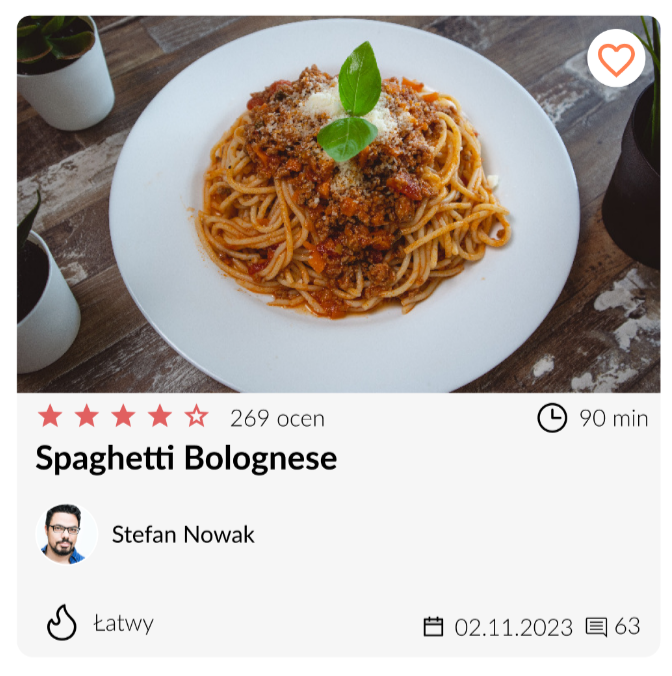
\includegraphics[width=0.4\textwidth]{images/review-item_1}
    \end{center}
    \caption{Karta prezentująca najważniejsze informacje o potrawie; możliwa do znalezienia na stronie głównej lub podstronie do wyszukiwania receptur}
    \label{fig:food_card}
\end{figure}

W prawym dolnym rogu znajduje się ikonka komentarzy pokazująca ile wpisów dostępnych jest o danym przepisie. Jedna z osób testujących zasugerowała, aby po kliknięciu w ową ikonkę
nastąpiło przekierowanie do sekcji komentarzy danego przepisu. Według nas jest to dobry pomysł, który zamierzamy wprowadzić w finalnej wersji produktu, ponieważ wydaje się
intuicyjny, a także oszczędza czas potencjalnego użytkownika.

\subsection{Oznaczenie wymaganych pół podczas dodawania nowego przepisu}
Jedna z osób, która testowała nasz interfejs nie była pewna czy musi dodawać zdjęcie do przepisu, a także czy wymagane jest uzupełnienie wszystkich pól. Nasz projekt w żaden 
sposób nie odpowiadał na te pytania. Stwierdziliśmy wspólnie z osobą testującą, że specjalne oznaczenie pól wymaganych znacznie podniosłoby czytelność interfejsu do dodawania
przepisów (często stosowanym zabiegiem przez wiele witryn internetowych, aby naprawić ten problem jest dodanie symbolu "*" obok wymaganych pól).

\subsection{Umożliwienie zaznaczenia kilku opcji w danej kategorii podczas filtrowania przepisów} 
Zaprezentowany prototyp nie przewidywał wybrania kilku opcji w rozwijanych menu na raz. Oznacza to, że użytkownik który chciałby wyświetlić zarówno przepisy, które nadają się
na obiad, jak i kolację musiałby wykonwać 2 osobne zapytania (jedno do wyświetlenia tylko dań obiadowych, a drugie tylko dla kolacyjnych). Podobnie jest w naszym prototypie 
dla pola z regionem pochodzenia, jak i dietą.

\subsection{Niepoprawne umieszczenie przypomnienia o konieczności zalogowania się}
\begin{figure}[H]
    \begin{center}
        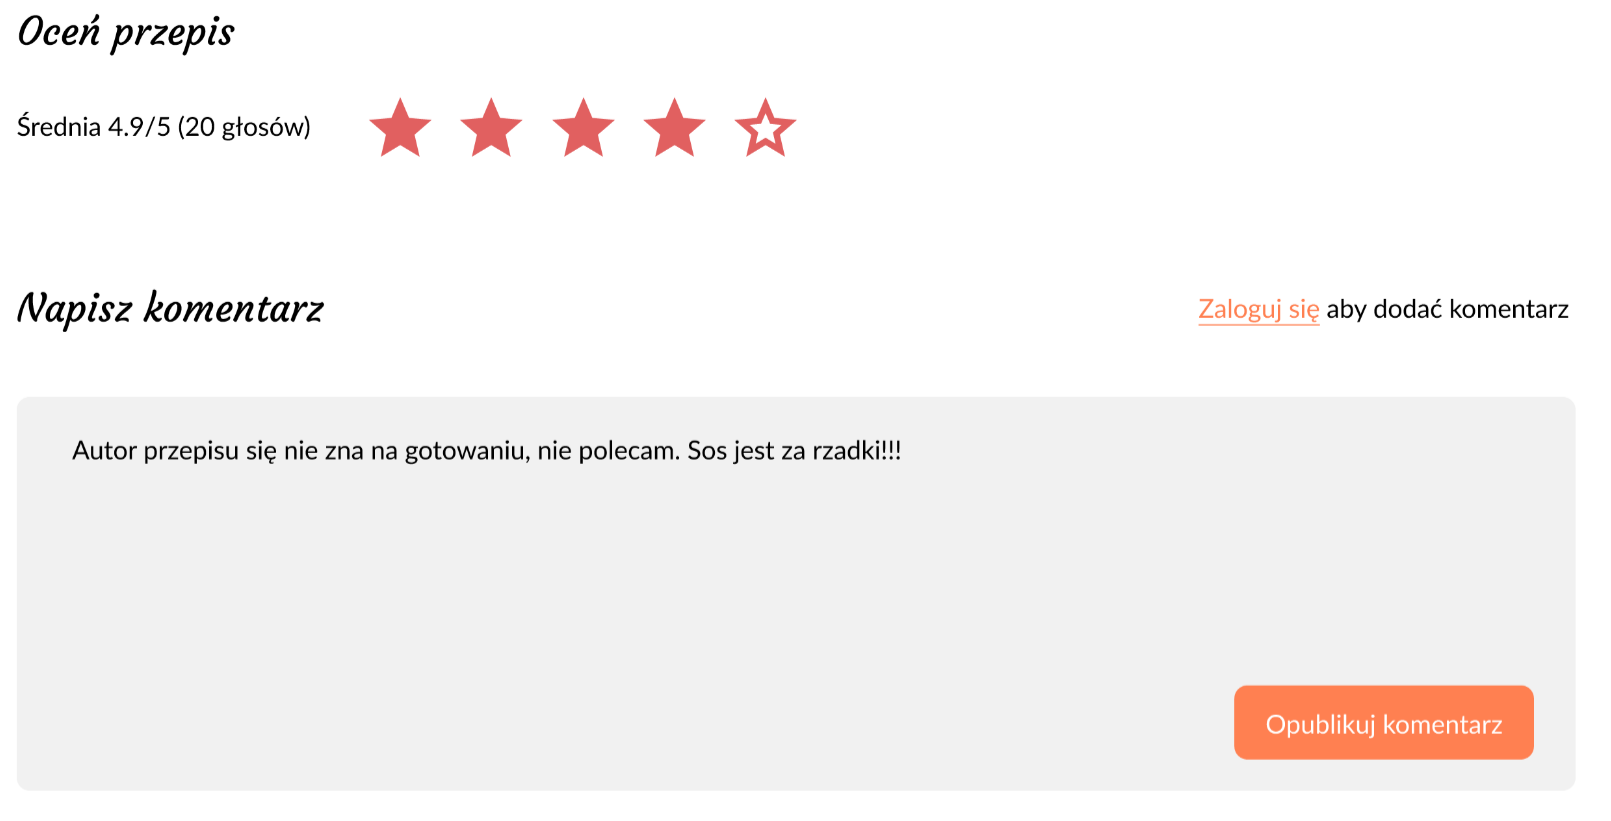
\includegraphics[width=0.8\textwidth]{images/review-item_2}
    \end{center}
    \caption{Fragment interfejsu, który ma umożliwiać komentowanie/ocenanie przepisów}
\end{figure}

W naszym oryginalnym zamyśle użytkownik miał mieć możliwość oceniania przepisu (z użyciem gwiazdek) lub/i zostawiania komentarza. Obie te czynności wymagają wcześniejszego zalogowania, ale
tylko w przypadku komentowania jest to jawnie powiedziane. Użytkownik widząc ekran z powyższego zdjęcia może odnieść wrażenie, że nie będąc zalogowanym można oceniać przepis (gwiazdeczki).
Wspólnie z testerami interfejsu ustaliliśmy, że lepiej byłoby umieścić informację o konieczności zalogowania się na wysokości już samych gwiazdek i przeredagować napis tak, aby było 
jasne, że w obu przypadkach jest to konieczne.

\subsection{Bardziej precyzyjne kategorie dotyczące regionu pochodzenia przepisu}
W obecnym stanie nasza aplikacja proponuje użytkownikowi do wyboru kontynenty, jako region pochodzenia danego przepisu. Jest to bardzo ogólny i nieprecyzyjny filtr, który powinien
być bardziej szczegółowy. Testerzy spodziewali się, że z pomocą tego filtra będą mogli zaznaczyć, że interesuje ich kuchnia polska lub włoska. Wspólnie ustaliliśmy, że powinniśmy 
umieścić tam opcje bardziej precyzyjne, związane z krajami a nie całymi kontynentami.

\subsection{Brakujące okienko dialogowe}
Przy tworzeniu prototypu strony do zarządzania naszym profilem zapomnieliśmy, aby po kliknięciu opcji "usuń profil" witryna pytała się czy na pewno chcemy wykonać tą akcję.
Dodanie tego okienka jest bardzo ważne, aby uniknąć przypadkowego usunięcia konta.

\section{Podsumowanie}
Proces testowania interfejsu na użytkownikach, którzy nie mieli z nim wcześniej do czynienia był bardzo przydatnym doświadczeniem. Pozwoliło to określić co może być poprawione
lub jakie elementy wymagają ponownego przemyślenia. Jak wspominałem wcześniej, wszystkie opinie były pozytywne, ale znalazło się kilka szczegółów, które wymagają drobnych poprawek.

\end{document}
